\section{Umsetzung}

\subsection{Technologieentscheidung}
\subsubsection{Versuchssystem}\label{sec:TechnologieVersuchssystem}
Aus der Konzeption in Kapitel~\ref{sec:Konzeption} gehen verschiedene Anforderungen an die Technologie hervor.
Durch die Verwendung von neuronalen Netzen werden die verfügbaren Technologien bzw. Programmiersprachen bereits eingeschränkt.
Um weitere Technologieenscheidungen zu treffen muss zunächst eine Programmiersprache ausgewählt werden.
Da in einer Umfrage unter Machine-Learning-Entwicklern und Data Scientists 57\% Python als Programmiersprache nutzen und 33\% diese sogar priorisieren, wird für dieses Projekt Python als Programmiersprache festgelegt \autocite[vgl. ][S. 16]{vision_mobile_state_2017}.
In einer allgemeinen Umfrage zu verwendeten Programmiersprachen liegt Python mit 49,2\% auf Platz drei \autocite[vgl.][]{yepis_2023_2023}.
Das bedeutet, dass knapp die Hälfte der befragten Entwickler unter anderem Python verwenden, somit ist eine ausreichende Verbreitung gewährleistet.
Die Verbreitung ist vor allem deshalb ein wichtiger Aspekt, da es durch eine hohe Verbreitung ein großes Eco-System mit vielen quelloffenen Ressourcen und bereits durchgeführten Projekten gibt.

Um Machine-Learning mit Python zu betreiben, gibt es mehrere Bibliotheken zur Auswahl.
Die 3 bekanntesten Open-Source-Bibliotheken sind dabei \gqq{TensorFlow}, \gqq{PyTorch} und \gqq{SciKit-Lern} \autocite[vgl.][]{msv_tensorflow_2020}.

Diese Bibliotheken sind sich relativ ähnlich.
Vorteile einer Bibliothek bringen automatisch auch Nachteile, die sich somit gegenseitig aufheben.

Der wesentliche Unterschied zwischen den Bibliotheken ist, dass die Entwickler dieser Studienarbeit bereits Vorkenntnisse in Tensorflow haben, weshalb Tensorflow verwendet wird.
Zusätzlich wird das Modul \gqq{Keras} verwendet, welches eine entwicklerfreundliche High-Level-Schnittstelle für Tensorflow ist und somit eine einfachere Entwicklung ermöglicht \autocite[vgl.][]{noauthor_keras_2023}.

\subsubsection{Demosystem}
Für die Technologieentscheidung muss zunächst zwischen den zwei Komponenten Client und Server unterscheiden werden.
Da für beide Teile unterschiedliche Anforderungen erfüllt werden müssen, erfolgt die Technologieentscheidung separat.
Außerdem findet eine Festlegung des verwendeten Protokolls für die Schnittstellenkommunikation statt.

\paragraph{Client}
Die grundlegende Anforderung an den Client ist die Umsetzung als Webapplikation.
Daraus leiten sich in erster Linie vier verschiedene Programmiersprachen ab: JavaScript/Type\-Script, Python, PHP und Ruby.

Für eine weitergehende Einschränkung ist der vorausgesetzte Funktionsumfang relevant.
Dieser ist sehr gering, da lediglich Input-Elemente für die Angabe eines zu authentifizierenden Sprechers, sowie zur Auswahl einer zu verwendeten Datei bereitgestellt werden müssen.
Außerdem muss eine Verbindung zu einem Back-End (Server) aufgebaut werden können.

Da diese Anforderungen durch alle vier Kandidaten erfüllt werden, muss die Entscheidung durch andere Kriterien erfolgen.
Hierbei spielen vor allem zwei Aspekte eine Rolle.
Eine Umfrage von Stack Overflow aus dem Jahr 2020 zeigt, dass JavaScript die beliebteste Programmiersprache von professionellen Entwickler ist.
Moderne Frameworks wie Reactjs und Angular haben die klassische Webprogrammierung in PHP über die letzten Jahre abgelöst \autocite[vgl.][]{stack_overflow_stack_2020}.

Da es sich außerdem um ein Demosystem handelt, welches lediglich die Ergebnisse dieser Arbeit präsentieren soll und somit nicht in einem produktiven Umfeld betrieben wird, spielt die Technologieentscheidung nur eine untergeordnete Rolle.
Die Kompetenzen des Entwicklerteams liegen vor allem im Bereich der React Programmierung mit JavaScript beziehungsweise TypeScript.

Zusammenfassend fällt die Technologieentscheidung für die Client Implementierung somit auf das JavaScript Framework Reactjs in Kombination mit TypeScript.
TypeScript ermöglicht dabei gegenüber JavaScript die Verwendung von Datentypen, wodurch Datentypfehler im Rahmen der Implementierung vermieden werden können.

\paragraph{Schnittstelle}
Im Web-Umfeld spielt das \ac{HTTP} eine besondere Rolle.
Dabei handelt es sich um ein zustandsloses Protokoll zur Übertragung von Daten auf der Anwendungsschicht.
Ein Anwendungsfall ist dabei die Anfrage von Websiten im Browser über die URL.
Dazu wird eine sogenannte \ac{HTTP}-GET Anfrage an den Zielserver gesendet, welcher anschließend mit der angeforderten Ressource antwortet.

Nach demselben Prinzip kann das HTTP Protokoll ebenfalls dazu verwendet werden, eine Kommunikation zwischen Client und Server zu ermöglichen.
Die zu übergebenden Variablen des Clients an den Server können dabei innerhalb der URL des GET-Requests übertragen werden.
Gleichzeitig können die Ergebnisse des Servers beispielsweise im JSON-Format an den Client zurückgesendet werden.

Da das HTTP Protokoll somit alle benötigten Anforderungen erfüllt, kommt es für die Schnittstellenkommunikation zum Einsatz.

\paragraph{Server}
Für den Authentifizierungsprozess implementiert der Server denselben Ablauf wie das Versuchssystem.
Um eine doppelte Entwicklung zu vermeiden, entsteht somit eine Abhängigkeit zwischen der Technologieentscheidung des Versuchssystems und des Servers.
Aus der Technologieentscheidung des Versuchssystems in Kapitel~\ref{sec:TechnologieVersuchssystem} geht die Programmiersprache Python hervor.
Somit sollte zunächst geprüft werden, ob die Anforderungen des Servers in der Sprache Python umsetzbar sind.

Neben dem Authentifizierungsprozess spielt ausschließlich die Schnittstellenkommunikation zwischen Client und Server eine Rolle für die Technologieentscheidung des Servers.
Da als Kommunikationsprotokoll HTTP eingesetzt wird, muss also eine Bibliothek gefunden werden, die die Verwendung dieses Protokolls in Python ermöglicht.
Hierzu kann Flask verwendet werden.

Bei Flask handelt es sich um ein Web Framework, welches eine Bereitstellung von \ac{API} Endpunkten, die über das \ac{HTTP} Protokoll abrufbar sind, ermöglicht.

Somit können alle Anforderungen an die Serverapplikation mittels der Programmiersprache Python umgesetzt werden.
Dazu können die bereits entwickelten Komponenten für den Authentifizierungsprozess aus dem Versuchssystem übernommen werden.

\subsection{Versuchssystem}

\subsubsection{Feature Kombination}
Wie bereits in Kapitel~\ref{sec:FeatureKombination} erwähnt müssen zuerst die Konfigurationen erzeugt werden.
Hierzu werden die vorher definierten Werte in einer JSON Datei erfasst und durch ein Tool alle möglichen Konfiguration mit einer ID erzeugt.
Hierbei muss beachtet werden, dass durch die Kombination Konfigurationen entstehen in welchen nichts berechnet werden muss.
Die erstellte JSON Datei ist in dem Listing~\ref{configs} dargestellt.
\begin{lstlisting}[language=JavaScript,numbers=none,caption=Konfigurationsmöglichkeiten,label=configs]
Configs = {
    "amount_of_frames": [10000, 15000],
    "size_of_frame": [400, 600],
    "LPC": {
        "order": [13, 20],
        "weight": [0, 1]
    },
    "MFCC": {
        "order": [13, 20],
        "weight": [0, 1]
    },
    "LPCC": {
        "order": [13, 20],
        "weight": [0, 1]
    },
    "delta_MFCC": {
        "order": [13],
        "weight": [0, 1]
    }
}
\end{lstlisting}
Der \codestyle{weight} Parameter gibt lediglich an, ob in dieser Konfiguration dieses Feature verwendet werden soll oder nicht.

\subsubsection{Datensatz}
Für die Evaluierung der Stimmmerkmale wird ein geeigneter Datensatz benötigt.
Hierzu wurde nach einer Internetrecherche auf der Plattform \gqq{Kaggle} ein entsprechender Datensatz gefunden, der die Anforderung aus Kapitel~\ref{sec:KonzeptDatensatz} erfüllt \autocite[vgl.][]{jain_speaker_2019}. 
Der Originaldatensatz enthält Audiodaten zu 50 Sprechern mit mindestens 60 Minuten Aufzeichnung pro Sprecher in mehreren kompressionslosen WAV Dateien.

In einem ersten Schritt müssen die Daten aufbereitet werden.
Der Originaldatensatz lässt sich in zwei Teile teilen, während der erste Teil aus YouTube Videos besteht, sind im zweiten Teil Aufnahmen von englischen Hörbüchern enthalten.
Da die Aufnahmequalität der Hörbücher deutlich besser ist, wurden nur diese Datensätze weiterverwendet.
In einem Folgeschritt werden die einzelnen Dateien der Datensätze zu einer Datei zusammengefügt und genauer betrachtet.
Hierbei konnten längere Pausen und Abweichungen der Datensätze, wie z.B. mehrere Sprecher oder eine andere Sprache identifiziert werden.
Diese Pausen wurden entfernt und die betroffenen Datensätze aus dem Datensatz entfernt.
Dadurch bleiben 25 geeignete Datensätze übrig, aus diesen wurden unter dem Aspekt des Geschlechts 20 Datensätze ausgewählt, sodass neun weibliche und elf männliche Sprecher im finalen Datensatz sind, da nur neun weibliche Datensätze geeignet sind.
Abschließend wurde für jeden Sprecher eine Audiodatei zum Trainieren des neuronalen Netzes mit acht Minuten erstellt und zur Evaluation 5 Sequenzen mit jeweils 15 Sekunden.
Das Testmaterial ist nicht im Trainingsmaterial enthalten.

\subsubsection{Vorverarbeitung und Feature Extraktion}

Um eine effektive Verarbeitung eines Audiosignals zu ermöglichen, muss zunächst eine Vorverarbeitung des Signals erfolgen (s. Kapitel~\ref{sec:preprocessing}).
Hierfür wird der Audio-Clip mittels der Bibliothek \gqq{Librosa} geladen.
Anschließend folgt der erste Schritt der Vorverarbeitung, das Entfernen von stillen Passagen.
Dafür wird ein selbst entwickelter Algorithmus verwendet, der erkennt, wenn sich die Amplitude des Audiosignals über einen gewissen Zeitraum unterhalb eines definierten Schwellwerts befindet.

\begin{lstlisting}[language=Python,numbers=none,caption=Remove Silence,label=lst-remove-silence]
for i, amp in enumerate(y):
if abs(amp) < threshold:
    counter_below_threshold += 1
else:
    if counter_below_threshold > pause_length_in_ms:
        for index in range(i-counter_below_threshold+keep_at_start_and_end, i-keep_at_start_and_end):
            indices_to_remove.append(index)
    counter_below_threshold = 0
\end{lstlisting}

Nach dem Entfernen der Pausen wird das Hintergrundrauschen entfernt.
Dafür wird ein externer Algorithmus von Tim Sainburg verwendet \autocite[][]{sainburg_timsainbnoisereduce_2019}.

Die abschließende Unterteilung des Audiosignals
in Frames, sowie das Windowing der Frames findet mit Hilfe von \codestyle{numpy}-Operationen in den Funktionen \codestyle{create_frames} und \codestyle{window_frames} statt.
Die passende Fensterfunktion wird dabei ebenfalls durch die \codestyle{numpy}-Bibliothek bereitgestellt.

Für das Extrahieren der Merkmale aus dem Audiosignal wird ein Ansatz gewählt, der eine einfache Erweiterung des Programms um verschiedene andere Verfahren ermöglicht.
Dazu wird das Designmuster Strategie in abgewandelter Form verwendet, wobei zunächst ein Interface für die Berechnungsverfahren erstellt werden muss.
Dieses definiert die Funktion \codestyle{calculate_features}, welche in den abgeleiteten Klassen implementiert wird.
Für die eigentlichen Berechnungen der Koeffizienten wird wieder die Signal-Verarbeitungs-Bibliothek Librosa verwendet.


Da für die Versuchsreihe sehr viele zeitaufwändige Berechnungen laufen müssen, ist das Extrahieren der Merkmale mit Multiprocessing implementiert.
Hierfür wird die python-interne Bibliothek \gqq{mutliprocessing} genutzt, um die Berechnung auf mehrere Threads zu verteilen.

% librosa load 
% remove silence 
% noice_reduce#

% berechnung der Merkmale für Trainings- und Testdaten --> benötigt für Traditionellen Authentifizierungsprozess

\subsubsection{Klassifikation und Evaluierung}
In dem Kapitel~\ref{sec:KonzeptKlassifikation} wurden neuronale Netze als Klassifikationsmodell gewählt, um die zuvor berechneten Merkmale zu evaluieren.
Hierbei werden zuerst neuronale Netze mit den berechneten Trainingsdaten trainiert, diese Netze bestehen aus drei Hidden-Layer mit jeweils 128, 64 und 32 Neuronen.
Dieser absteigende Aufbau stellt sich bei Versuchen als geeignete Lösung heraus.
Wie bereits im Konzept dargestellt müssen mehrere neuronale Netze trainiert werden, in diesem Fall werden für jede Konfiguration drei neuronale Netze erstellt.

\begin{lstlisting}[language=Python,numbers=none,caption=Erstellen und Trainieren eines neuronalen Netzes,label=lst-nn]
# create model
tf.keras.backend.clear_session()
model = tf.keras.models.Sequential([
    tf.keras.layers.Flatten(input_shape=[input_layer_neurons]),
    *hidden_layer, # 128, 64, 32
    tf.keras.layers.Dense(output_layer_neurons, activation=tf.nn.softmax),
])
model.compile(optimizer=tf.optimizers.Adam(), loss='sparse_categorical_crossentropy', metrics=['accuracy'])

# train model
model.fit(X, y, epochs=epochs)
\end{lstlisting}

Nach dem Training erfolgt die Evaluation der neuronalen Netze, hierzu wird der tatsächliche Authentifizierungsprozess nachgebildet.
Die berechneten Testdaten werden auf die neuronalen Netze angewandt, das neuronale Netz klassifiziert also die Daten indem es die Features jedes Frames einem der 20 Sprecher zuordnet.
Die Anzahl der Frames ist dabei von der Frame-Länge der jeweiligen Konfiguration abhängig, weshalb die Zuordnungsverteilungen normiert, also von einer absoluten in eine relative Zuordnung umgerechnet werden müssen.

Da für jeden Sprecher fünf Testdateien vorliegen entstehen pro neuronalem Netz 100 Zuordnungsverteilungen.
Durch die Berechnung von drei neuronalen Netzen pro Konfiguration ergibt dies 300 Zuordnungsverteilungen pro Konfiguration.

Nach Abschluss der Klassifikation aller Features können diese Datensätze ausgewertet werden und somit ein Rückschluss auf die beste Merkmalskombination getroffen werden.
Die Durchführung und Evaluation des Versuchs sind in Kapitel~\ref{sec:Evaluation} dargestellt.

\subsection{Demosystem}
Die Umsetzung von Client und Server ist im Folgenden kurz beschrieben.
Dabei werden lediglich die wichtigsten Aspekte benannt.
Da der Authentifizierungsablauf bereits im vorangehenden Kapitel erläutert wurde, wird in der Umsetzung des Servers nicht mehr darauf eingegangen.

\subsubsection{Client}
Die im Client implementierte Benutzeroberfläche zeigt eine Login-Abfrage (siehe Abbildung~\ref{fig:AppLogin}).
Diese unterteilt sich in zwei Abschnitte.
Zunächst kann über ein Eingabefeld die ID des zu authentifizierenden Nutzers angegeben werden.
Anschließend kann eine zu verwendende Audiodatei aus einer Liste ausgewählt werden.
Dabei stehen für jeden Nutzer mindestens fünf verschiedene Dateien zur Verfügung.
Um die Benutzerfreundlichkeit zu verbessern besteht dabei zusätzlich die Möglichkeit, die ausgewählte Datei im Browser abzuspielen.
Dafür wird der HTML \textFunktion{<audio>} tag verwendet.
\begin{figure}[H]
    \begin{subfigure}[c]{0.49\textwidth}
        \centering
        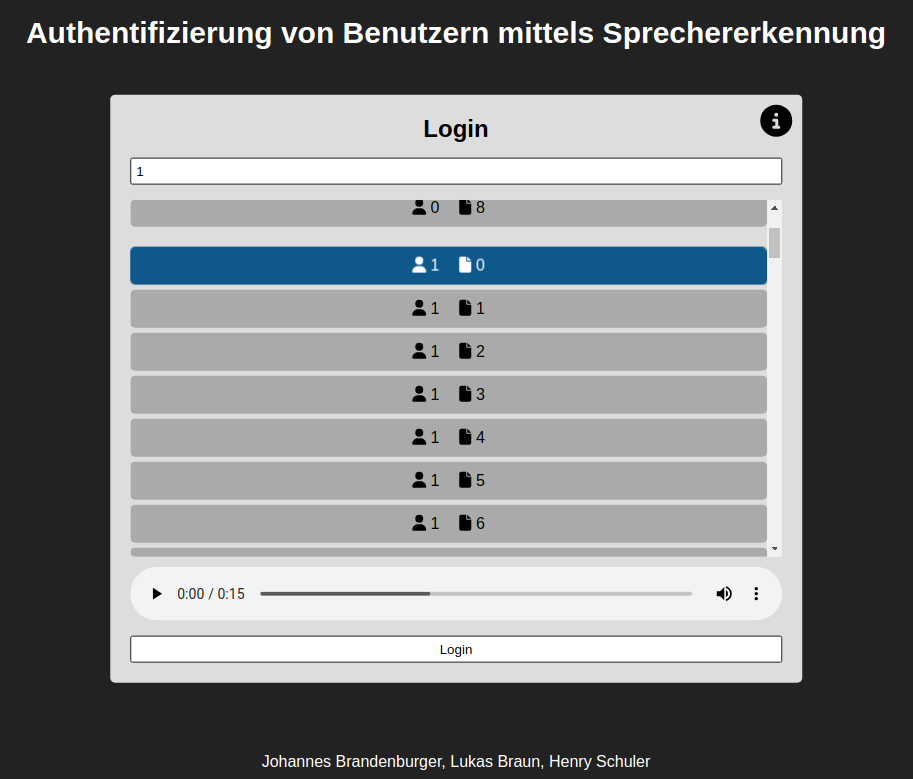
\includegraphics[width=0.9\textwidth, keepaspectratio]{images/UI.png}
        \subcaption{App/Login}
        \label{fig:AppLogin}
    \end{subfigure}
    \begin{subfigure}[c]{0.49\textwidth}
        \centering
        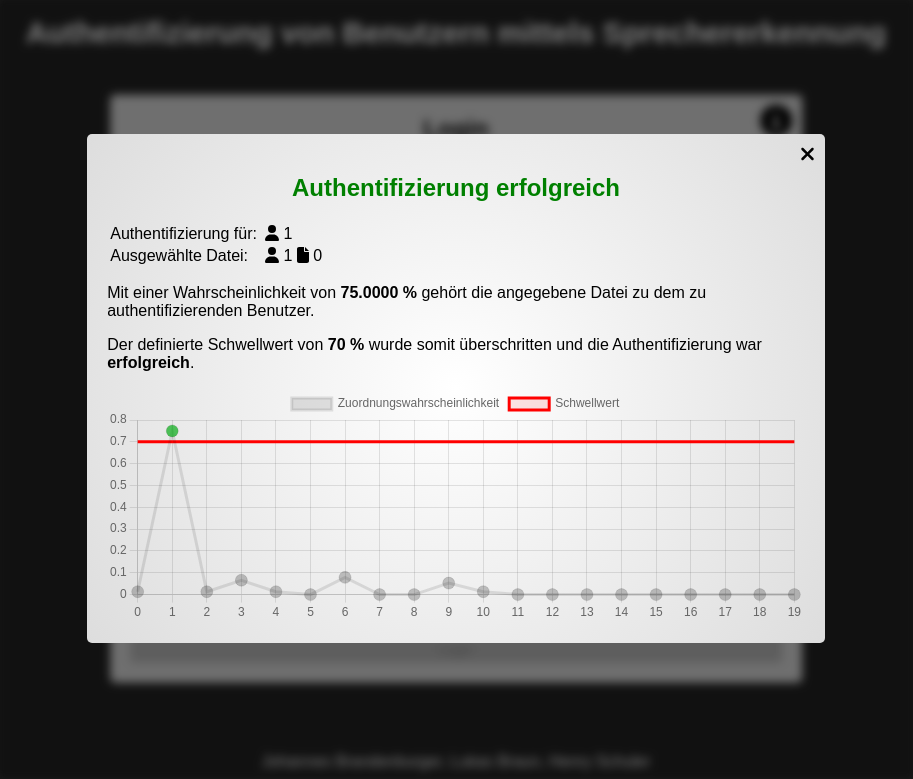
\includegraphics[width=0.9\textwidth, keepaspectratio]{images/UIResult.png}
        \caption{Result}
        \label{fig:Result}
    \end{subfigure}
    \caption{Weboberfläche}
\end{figure}
Über den Login-Knopf wird die Authentifizierungsanfrage an den Server gesendet.
Dafür wird die \textFunktion{fetch()} Funktion von JavaScript verwendet.
Die zu übergebenden Parameter werden als URL-Parameter angegeben.

Die Darstellung des Ergebnisses mittels der \textKlasse{Result} Komponente ist in Abbildung~\ref{fig:Result} dargestellt.
Dem Benutzer werden sowohl seine Authentifizierungsangaben, als auch das Ergebnis der Authentifizierung in Textform angezeigt.
Die Klassifikation als \gqq{erfolgreich} oder \gqq{fehlgeschlagen} kann sowohl dem Text als auch der Farbe der Überschrift (grün oder rot) entnommen werden.

Zusätzlich erhält der Benutzer einen grafischen Einblick in die Wahrscheinlichkeitsverteilung der Zuordnung der ausgewählten Sprecherdatei zu den verschiedenen Sprechern.
Das Diagramm wird mit Hilfe der Bibliotheken chart.js und react-chartjs-2 eingebunden.

\subsubsection{Server} 
Wie in der Technologieentscheidung bereits erwähnt, wird der Server mit Hilfe der Bibliothek Flask implementiert.
Listing~\ref{lst:serverPy} zeigt dabei die wesentlichen Codeabschnitte für die Umsetzung des Servers als Flask Applikation.
\begin{lstlisting}[language=Python,numbers=none,caption=Ausschnitt server.py,label=lst:serverPy]
    app = Flask(__name__)
    CORS(app)

    @app.route("/", methods=["GET", "POST"])
    def handle_api_request():
        ...

    if __name__ == '__main__':
        app.run(debug=False, host='127.0.0.1', port=5500)
\end{lstlisting}
Zunächst muss eine neue Flask \textVariable{app} erstellt werden.
Mittels \textFunktion{CORS(app)} wird dabei sichergestellt, dass eine Verbindung zwischen Client und Server trotz unterschiedlichem Ursprung möglich ist.

Die Authentifizierungsfunktion wird über die Wrapper-Funktion \textFunktion{handle\_api\_request()} und dem Decorator \textFunktion{@app.route()} als \ac{API} Endpoint verfügbar gemacht.

Abschließend kann der Server über die Anweisung \textFunktion{app.run()} unter Angabe der IP-Adresse und des Ports gestartet werden.

Das neuronale Netz, welches vom Server für die Authentifizierung von Benutzern verwendet wird, ergibt sich aus der Evaluation des Versuchssystems im nachfolgenden Kapitel~\ref{sec:Evaluation}.
Hierzu wird mit der ermittelten Konfiguration ein neues neuronales Netz trainiert, unter Verwendung von einer erhöhten Anzahl an Epochen, um die Genauigkeit des Systems noch einmal zu verbessern.
Vorgreifend muss hierbei erwähnt werden, dass das System durch die Erhöhung der Epochen in so fern verbessert werden konnte, dass die Grenze für die Anzahl an Frames die dem zu authentifizierenden Nutzer zugeordnet werden müssen, von 65 \% auf 70 \% erhöht werden kann.
Deshalb zeigt die Abbildung~\ref{fig:Result} in der Wahrscheinlichkeitsverteilung einen Threshold von 70 \%.
